\section{Proposed Scheme}
\label{sec:proposed-scheme}

% \begin{figure}[tb]
% \centering
%   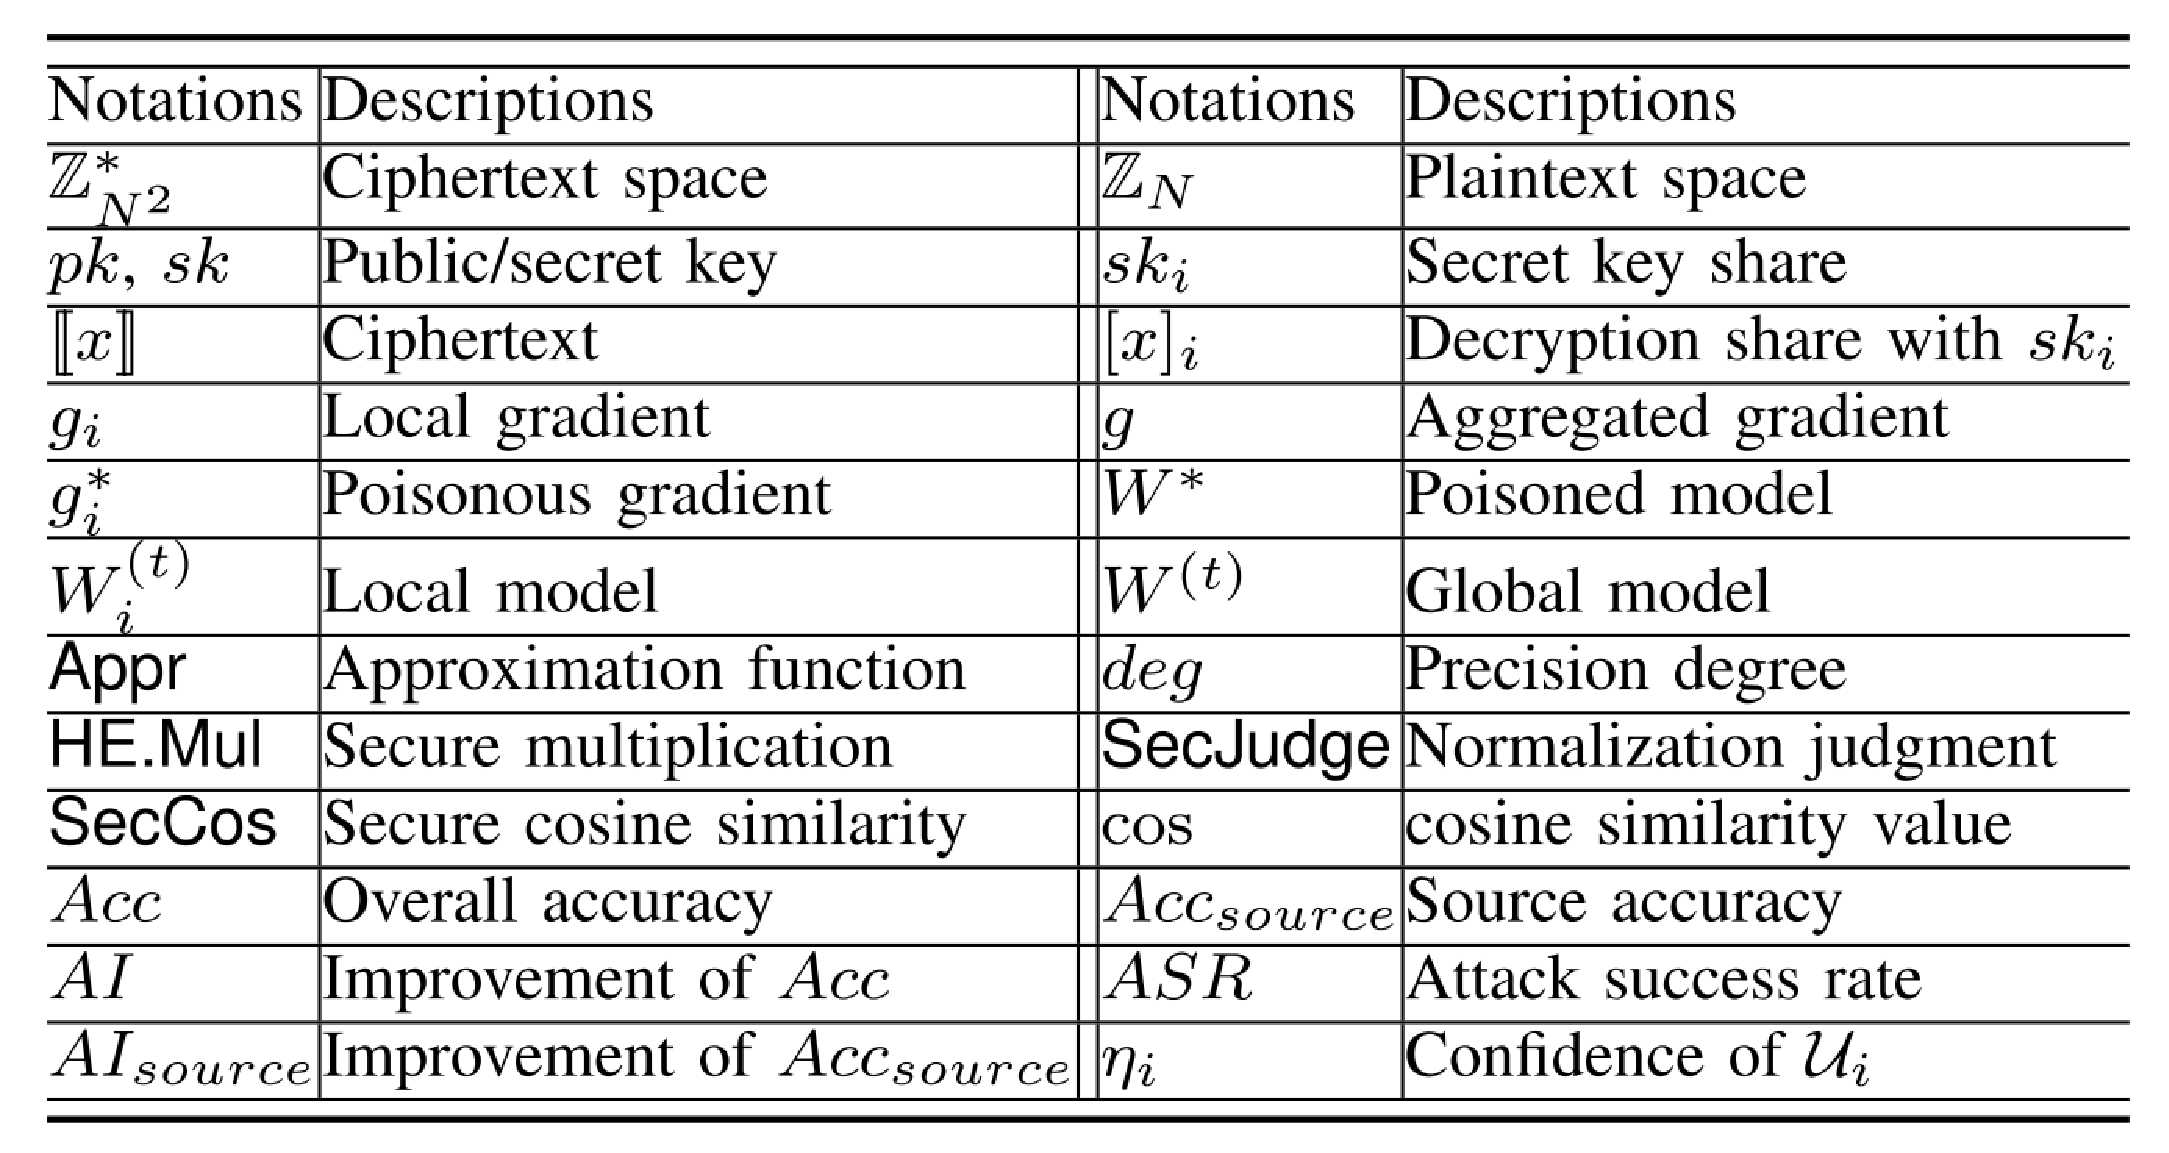
\includegraphics[width=0.8\linewidth]{resources/notations.pdf}
%   \caption{Notations}
%   \label{fig:notations}
%   %\vspace{-5mm}
% \end{figure}

% \Cref{fig:notations} summarizes the important notations used in the paper.
ShieldFL works with both IID and non-IID data.
In the former, the training data are uniformly partitioned among the users, while the latter, the training data is divided by class, where each user stores training data samples belonging to a single class.
In addition, shieldFL relies on two-trapdoor HE, described in \Cref{sec:preliminary-he}.
To protect against not normalized gradients, $SecJudge$ is proposed as a normalization judgment function.
More over, since the local gradients are encrypted $[[g_i^{(t)}$, $SecCos$ function is proposed to implement the secure cosine similarity between two encrypted gradients, which employs $HE.Mul$ function, explained in \Cref{app:he-multiplication}.
% If  a local gradient is dissimilar from an aggregated gradient, it is more likely to be poisonous, as shown in \Cref{fig:malicious-gradients-example}.

% \begin{figure}[htb]
% \centering
%   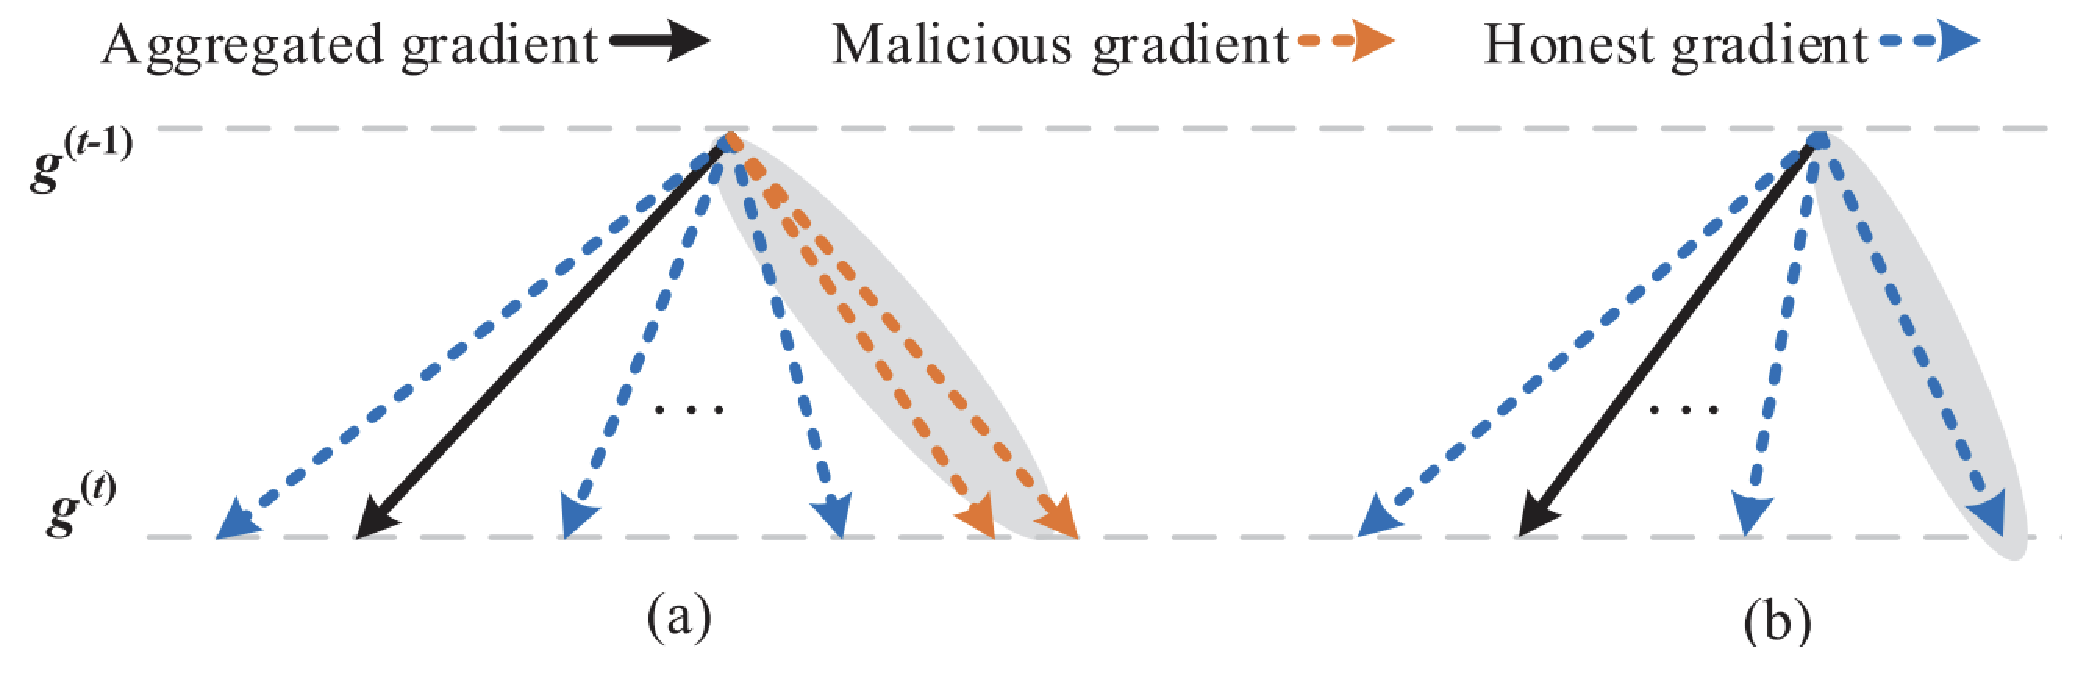
\includegraphics[width=0.8\linewidth]{resources/malicious-gradients-example.pdf}
%   \caption{Malicious gradients example}
%   \label{fig:malicious-gradients-example}
%   %\vspace{-5mm}
% \end{figure}

ShieldFL consists of three main algorithms: setup, local training, and privacy-preserving defense strategy.
The setup algorithm in \Cref{fig:setup-algo} is executed by the Key center to generate the keys to be used by the servers $S_1, S_2$ and the users $U_i$s.
First it splits the $sk$ between the two servers (Line 3).
It also splits the $sk$ between the first server $S_1$ and every user $U_i$ (Lines 4-5).
Finally, each user using his share of the key $sk_{s_i}$ to decrypt the encrypted initial weights $[[W^{(0)}]]$, that they will use as seed weights to start the training from.
We emphasize that the HE operations are explained in \Cref{sec:preliminary-he}.

\begin{figure}[htb]
\centering
  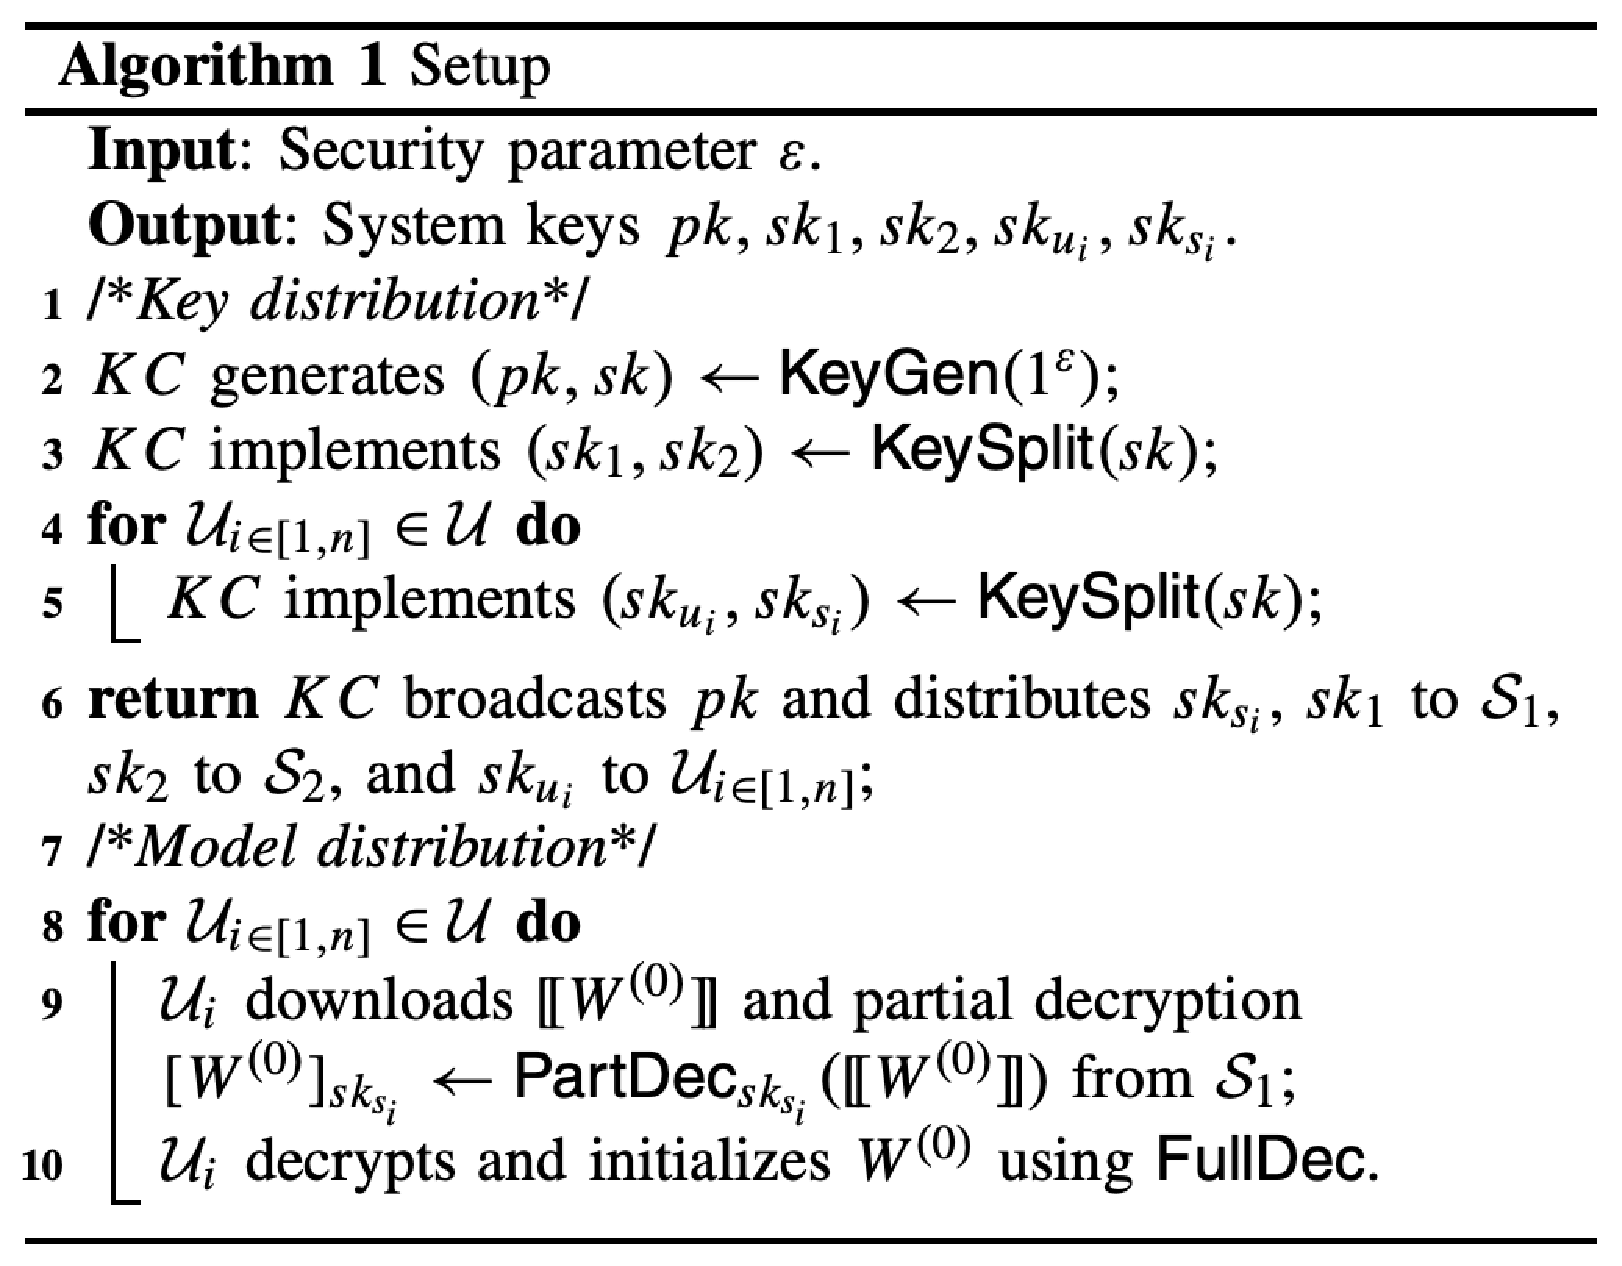
\includegraphics[width=0.8\linewidth]{resources/setup-algo.pdf}
  \caption{Setup algorithm}
  \label{fig:setup-algo}
  %\vspace{-5mm}
\end{figure}

Each user executes the local training algorithm (\Cref{fig:local-training-algo}) on its own private data $D_i$ to generate private gradients $g_i^{(t)}$.
Then, the user $U_i$ encrypts this gradient $[[g_i^{(t)}]]$ and shares it with the $S_1$.
To be specific, each user encrypts the gradients as follows: $[[g_i^{(t)}]] = \{ [[x'_1]], [[x'_2]], ..., [[x'_m]]\}$, and $[[x']] \leftarrow Enc_{pk}(x')$, where $x' \in g_i^{(t)}$.
On the other hand, if the user is malicious, he generates poisoned encrypted gradients $[[g_i^{(*t)}]]$.

\begin{figure}[htb]
\centering
  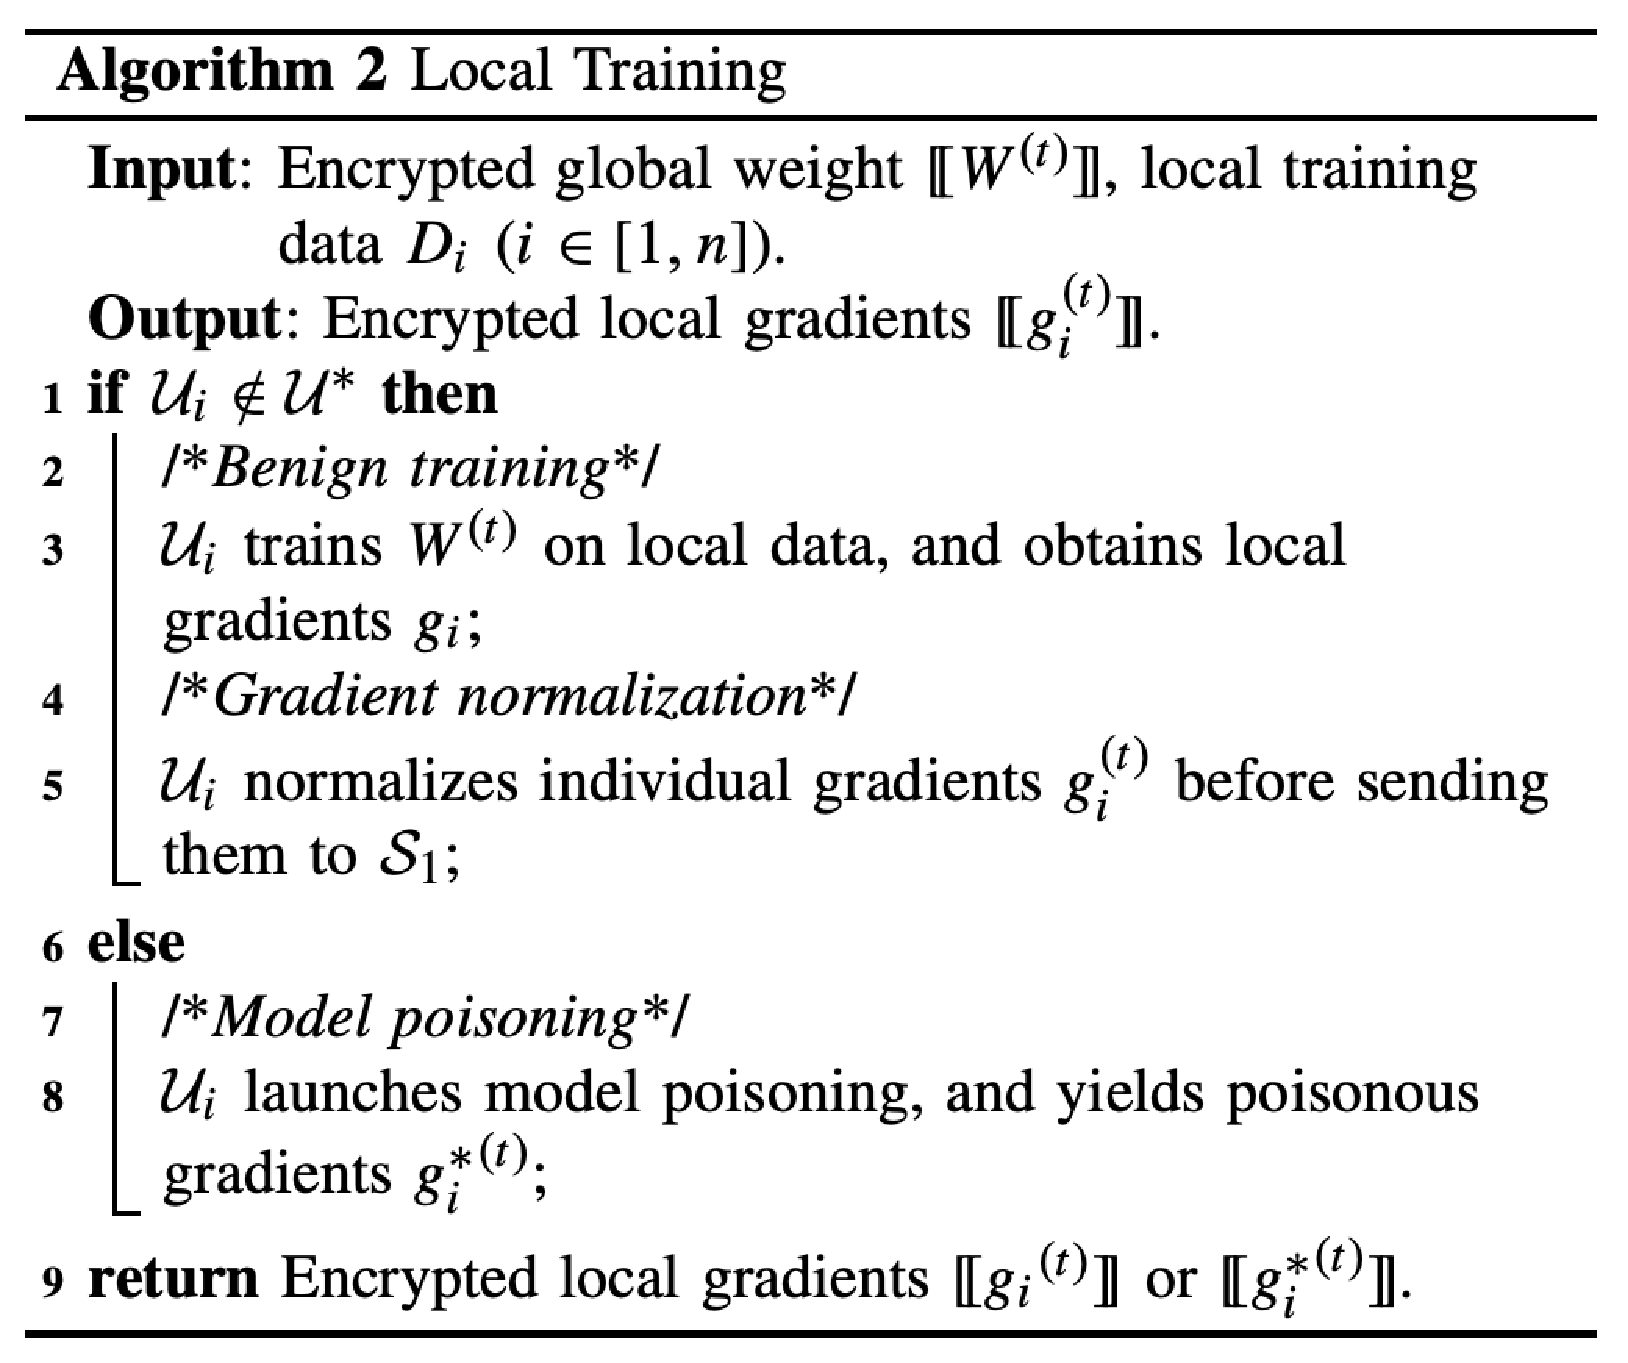
\includegraphics[width=0.8\linewidth]{resources/local-training.pdf}
  \caption{Local training algorithm}
  \label{fig:local-training-algo}
  %\vspace{-5mm}
\end{figure}

The server $S_1$ collects the encrypted gradients from all users, then executes the privacy-preserving defense strategy algorithm (\Cref{fig:privacy-preserving-defense-strategy-algo}), which generates the aggregated non-poisonous gradient $[[g^{(t)}]]$.
Lines 1–3 are executed in the case of the first training iteration, where it multiplies all the gradients it received from all users, which is equivalent to adding all the gradients together, as explained in \Cref{sec:preliminary-he}.
In addition, it calls the $HE.Trun$ algorithm that divides the sum over the number of users.
In line 6, $S_1$ executes the $SecJudge$ algorithm per user to judge if the reported gradient by that user is normalized or not.
If it is normalized, it reports their summation; otherwise, it aborts.
Lines 7-9 are executed only if the gradient reported by the user is normalized.
In line 9, it calculates the cosine similarity between the gradient reported by the user $[[g_i^{(t)}]]$ and the average gradient in the previous epoch $[[g^{(t-1)}]]$.
The smaller the value, the higher the similarity.
In line 10, the algorithm identifies the gradient with the highest cosine similarity, the farthest from the average gradient in the previous iteration, as the baseline for the poisonous gradient $g^*$.
Based on that, it recalculates the consine similarity once more for each gradient submitted by the users: $[[g_i^{(t)}]]$, and calculates the difference between this gradient and the baseline poisonous gradient $g^*$.
This time, the higher the value, the closer this gradient is to the poisonous gradient, and then it should be given a low confidence level, as shown in line 15.
Vice versa, the smaller the cosine value, the farther this gradient is from the baseline poisonous gradient, and then it should be given a high confidence level.
Finally, in line 18, the averaged gradient for this iteration is calculated as $g^{(t)} = [[g^{(t)}_1]]^{\eta_1} . [[g^{(t)}_2]]^{\eta_2} . [[g^{(t)}_n]]^{\eta_n} = [[g^{(t)}_1 . \eta_1 + g^{(t)}_2 . \eta_2 + ... g^{(t)}_n . \eta_n]]$.

\begin{figure}[htb]
\centering
  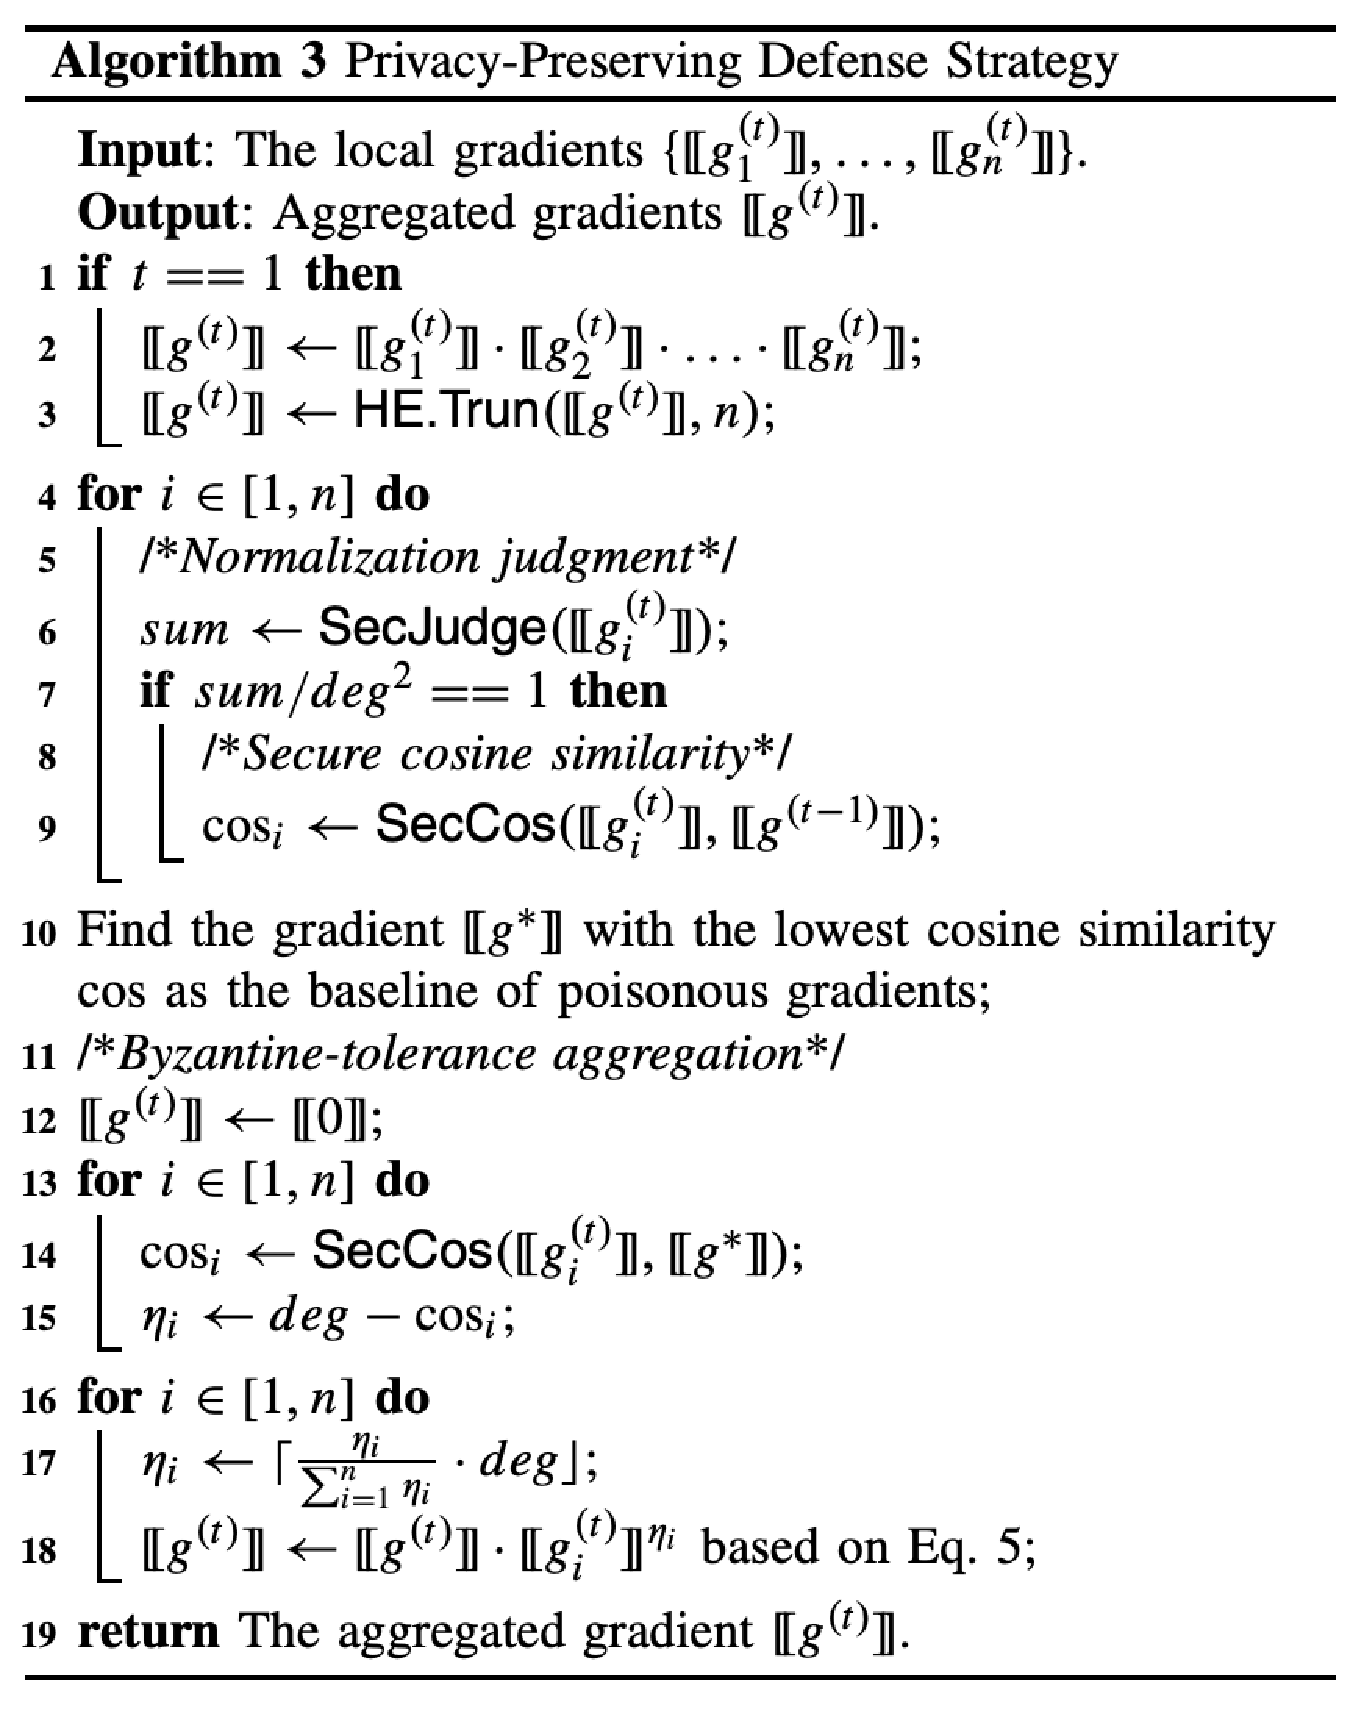
\includegraphics[width=0.8\linewidth]{resources/privacy-preserving-defense-strategy-algo.pdf}
  \caption{Privacy-preserving defense strategy algorithm}
  \label{fig:privacy-preserving-defense-strategy-algo}
  %\vspace{-5mm}
\end{figure}

Finally, the details of the $SecJudge$ and $SecCos$ implementations are discussed in \cref{app:normalization-judgement} and \Cref{app:cos-similarity}, respectively.
